\documentclass{article}
\usepackage[margin=1in]{geometry}
\usepackage{amsmath,amsfonts,amssymb}
\usepackage{listings}
\usepackage{color}
\usepackage{graphicx}
\usepackage{subfig}
\usepackage{blkarray}
\usepackage{multirow}
\usepackage{float}
\usepackage{caption}
\usepackage{subcaption}
\begin{document}
\begin{titlepage}
	\setlength{\parindent}{0pt}
	\large

\vspace*{-2cm}

\definecolor{dkgreen}{rgb}{0,0.6,0}
\definecolor{gray}{rgb}{0.5,0.5,0.5}
\definecolor{mauve}{rgb}{0.58,0,0.82}

\lstset{frame=tb,
  language=Python,
  aboveskip=3mm,
  belowskip=3mm,
  showstringspaces=false,
  columns=flexible,
  basicstyle={\small\ttfamily},
  numbers=none,
  numberstyle=\tiny\color{gray},
  keywordstyle=\color{blue},
  commentstyle=\color{dkgreen},
  stringstyle=\color{mauve},
  breaklines=true,
  breakatwhitespace=true,
  tabsize=3
}

University of Waterloo \par
CS 480 \par
\vspace{0.05cm}
r2knowle: 2023-10-22
\vspace{0.2cm}

{\huge Exercise \# 4 \par}
\hrule

\vspace{0.5cm}
\textbf{Q1)} Below are the graphs for the training and test accuracy for the different loss functions for the decision tree:
\begin{figure}[!htb]
    \centering
    \begin{minipage}{.5\textwidth}
        \centering
        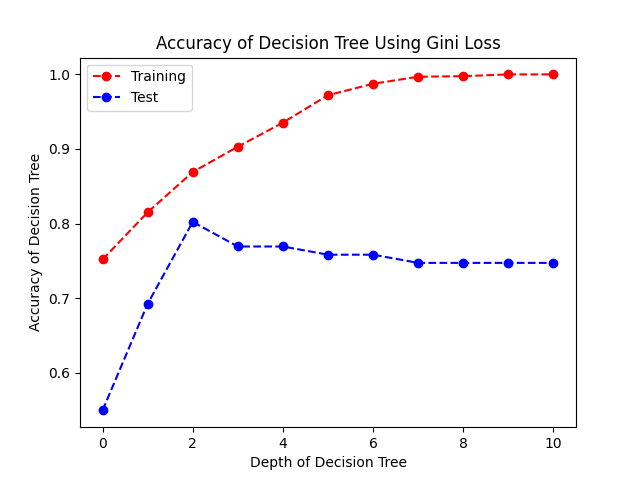
\includegraphics[width=\textwidth]{g1.png}
    \end{minipage}%
    \begin{minipage}{0.5\textwidth}
        \centering
        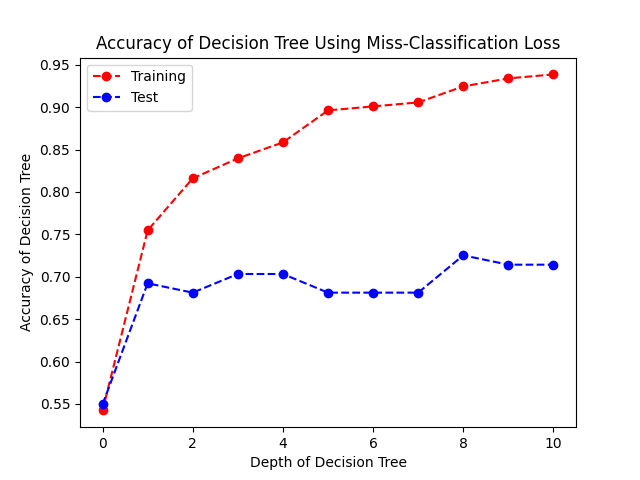
\includegraphics[width=\textwidth]{g2.png}
    \end{minipage}
\end{figure}
\begin{figure}[!htb]
    \centering
    \begin{minipage}{.5\textwidth}
        \centering
        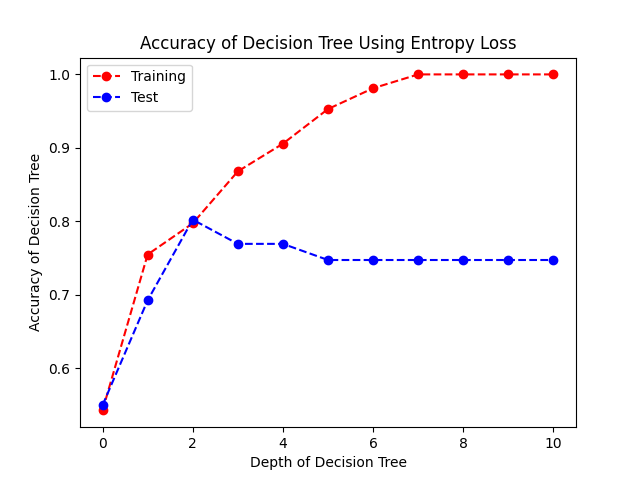
\includegraphics[width=\textwidth]{g3.png}
    \end{minipage}%
\end{figure} \\\\
What we see is that as the depth of the tree increase our training accuracy will increase too. Due to the fact that the higher the depth is the more over fitting we have means that the test accuracy will decrease past a certain point. Thus we see that increasing tree depth improves test accuracy up to a point and decreases test accuracy afterwards. \\
Conversely we see that each of the loss functions converge to the same rough test accuracy of $75\%$. Misclassification error seem to converge to this point as quick as possible, but gini loss and entropy loss reach the highest test accuracy of $80\%$.
\newpage
\textbf{Q2)} Below are the minimum, maximum and average test accuracy for bagging and random forest:
\[
\begin{tabular}{||c | c c c||} 
 \hline
  & \text{Min Test Accuracy} & \text{Max Test Accuracy} & \text{Median Test Accuracy} \\ [0.5ex] 
 \hline\hline
 \text{Random Forest} & 81.318\% & 84.615\% & 82.417\% \\ 
 \hline
 \text{Bagging} & 84.615\% & 87.912\% & 86.813\% \\
 \hline
\end{tabular}
\]
From what we can see, bagging seems to preform alot better as the variance in random forest seems to push down the mean. From these results we would expect that bagging preforms better then random forest.\\\\
However both of these out preform any of the other decision trees discussed in question 1, proving that ensamble methods tend to be more accurate then a solo decision tree classifier.
\newpage
\begin{lstlisting}
import pandas as pd
import numpy as np
import matplotlib.pyplot as plt
from sklearn import tree

# ============= Loss functions =============


def missClassLoss(vals_y):
    count = 0.0
    for val in vals_y:
        if val > 0:
            count += 1.0
    p = 0
    if count != 0:
        p = count / float(len(vals_y))

    return min(p, 1 - p)


def giniLoss(vals_y):
    count = 0.0
    for val in vals_y:
        if val > 0:
            count += 1.0
    p = 0
    if count != 0:
        p = count / float(len(vals_y))

    return p * (1 - p)


def entropyLoss(vals_y):
    count = 0.0
    for val in vals_y:
        if val > 0:
            count += 1.0
    p = 0
    if count != 0:
        p = count / float(len(vals_y))
    if p == 1 or p == 0:
        return 0
    return -p * np.log2(p) - (1 - p) * np.log2(1 - p)


# ============= Decision Tree Implementation =============
class DecisionTree:
    threshold = 0
    thresholdFeature = 0

    storedLabels = []

    leftTree = -1
    rightTree = -1

    classification = 0

    numLeft = 0
    numRight = 0

    counter = 0;
    def getLoss(self, loss):
        if self.leftTree == -1:
            return loss(self.storedLabels)
        else:
            leftLoss = self.leftTree.getLoss(loss) * self.numLeft/(self.numLeft+self.numRight)
            rightLoss = self.rightTree.getLoss(loss) * self.numRight/(self.numLeft+self.numRight)

            return leftLoss + rightLoss



    def findBestThreshold(self, vals_x, vals_y, loss):
        bestLoss = 9999999
        bestFeature = 0
        bestThreshold = 0

        rows, width = vals_x.shape
        for idx in range(0, rows):
            for param in range(0, width):
                left = []
                right = []
                for testidx in range(0, rows):
                    if vals_x[param][testidx] <= vals_x[param][idx]:
                        left.append(vals_y[testidx])
                    else:
                        right.append(vals_y[testidx])

                leftWeight = len(left) / (len(left) + len(right))
                rightWeight = len(right) / (len(left) + len(right))

                totalLoss = loss(left) * leftWeight + loss(right) * rightWeight
                if totalLoss < bestLoss:
                    bestLoss = totalLoss
                    bestFeature = param
                    bestThreshold = vals_x[param][idx]

        return [bestFeature, bestThreshold]

    def __init__(self, vals_x, vals_y, loss, depth):
        if depth == 0 or (len(vals_y) <= 1):
            if np.mean(vals_y) >= 0.5:
                self.classification = 1

            self.storedLabels = vals_y

        else:
            x = self.findBestThreshold(vals_x, vals_y, loss)

            self.thresholdFeature = x[0]
            self.threshold = x[1]

            lefty = []
            righty = []

            rows, width = vals_x.shape
            for idx in range(0, rows):
                if vals_x[self.thresholdFeature][idx] <= self.threshold:
                    lefty.append(vals_y[idx])
                else:
                    righty.append(vals_y[idx])

            if len(lefty) != 0 and len(righty) != 0:
                leftx = vals_x[vals_x[self.thresholdFeature] <= self.threshold]
                rightx = vals_x[vals_x[self.thresholdFeature] > self.threshold]

                leftx.reset_index(inplace=True, drop=True)
                rightx.reset_index(inplace=True, drop=True)

                self.numLeft = len(lefty)
                self.numRight = len(righty)

                self.leftTree = DecisionTree(leftx, lefty, loss, depth-1)
                self.rightTree = DecisionTree(rightx, righty, loss, depth-1)
            else:
                if np.mean(vals_y) >= 0.5:
                    self.classification = 1

                self.storedLabels = vals_y

    def classify(self, item_x, item_y):
        if self.leftTree == -1:
            self.counter += 1
            if item_y[0] == self.classification:
                return 1
            return 0
        else:
            if item_x[self.thresholdFeature] <= self.threshold:
                return self.leftTree.classify(item_x, item_y)
            return self.rightTree.classify(item_x, item_y)


    def predict(self, items_x, items_y):
        count = 0

        for i in range(0, items_x.shape[0]):
            count += self.classify(items_x.iloc[i], items_y.iloc[i])
        return( count/len(items_y) )


train_x = pd.read_csv("datasets/X_train_D.csv", header=None)
train_col_y = pd.read_csv("datasets/y_train_D.csv", header=None)
train_y = []

for val in range(0, train_col_y.shape[0]):
    train_y.append(train_col_y[0][val])

test_x = pd.read_csv("datasets/X_test_D.csv", header=None)
test_y = pd.read_csv("datasets/y_test_D.csv", header=None)

trainingLoss = []
testAccuracy = []
xAxis = []
for depth in range(0, 11):
    print(depth)
    dt = DecisionTree(train_x, train_y, entropyLoss, depth)
    trainingLoss.append(dt.predict(train_x, train_col_y))
    testAccuracy.append(dt.predict(test_x, test_y))
    xAxis.append(depth)

plt.plot(xAxis, trainingLoss, 'ro--', label="Training")
plt.plot(xAxis, testAccuracy, 'bo--', label="Test")
plt.legend()
plt.xlabel("Depth of Decision Tree")
plt.ylabel("Accuracy of Decision Tree")
plt.title("Accuracy of Decision Tree Using Entropy Loss")
plt.show()
\end{lstlisting}
\end{titlepage}
\end{document}